\par
Здесь приведены результаты работы алгоритма определения фазового состава на шести датчиках одного прибора скважины T1, описанной в части 2. Далее изображения пронумерованы следующим образом:
\begin{enumerate}[label=(\alph*)]
	\item
	Изначальные данные, преобразованные в выбранных координатах. Изображения (a)-(e) демонстрируют те же данные с различной раскраской.
	\item
	Тепловая карта данных, сделанная для демонстрации плотности точек.
	\item
	Полученная дискретная кластеризация данных на три фазы: «вода» (синий цвет), нефть (зеленый цвет) и газ (красный цвет).
	\item
	Полученная кластеризация с оценкой фазового состава в точках смены фаз. Желтый цвет указывает зоны смены фаз, остальные цвета соответствуют раскраске на (c). Для демонстрации везде выбраны значения порогов $$thr_{water}^1=thr_{oil}^1=0.99,\quad thr_{oil}^2=thr_{gas}^2=0.8$$ 
	\item
	Экспертная разметка для данного датчика. Цвета соответствуют (c).
	\item
	Матрица ошибок для оценки качества кластеризации (c) в сравнении с экспертной разметкой (e). В ячейках – количество точек, соответствующих произвольной комбинации «предсказанная метка – истинная метка».
	\item
	Матрица ошибок, построенная аналогично матрице (f), но значения отнормированы по строке.
\end{enumerate}
\par
Видно, что для датчика 3 не удалось достичь хороших результатов – в выбранных координатах не видно четко выраженных кластеров.

\newpage
\begin{figure}[H]
\centering
\subfloat[]{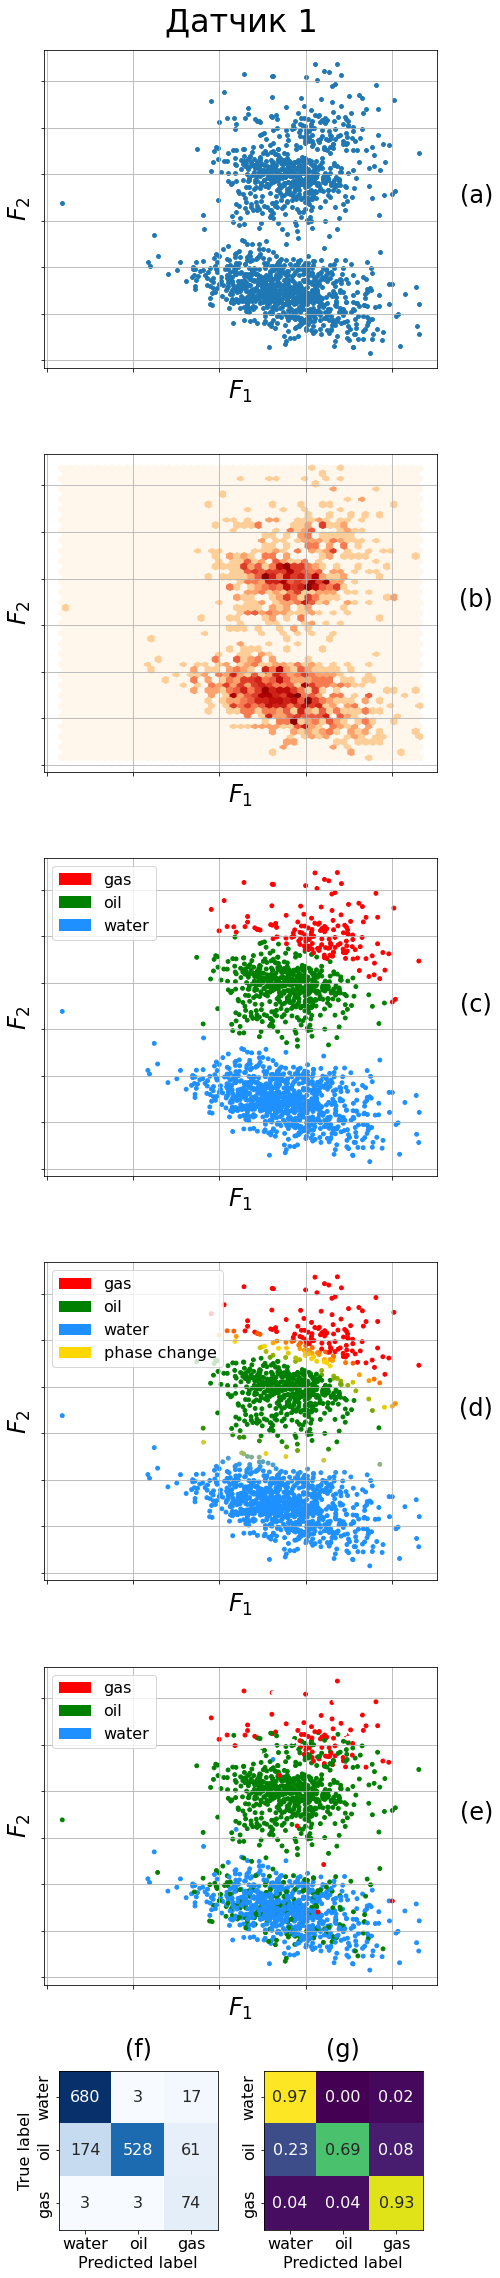
\includegraphics[width=0.3\textwidth]{TA/appendix_1.png}}
\subfloat[]{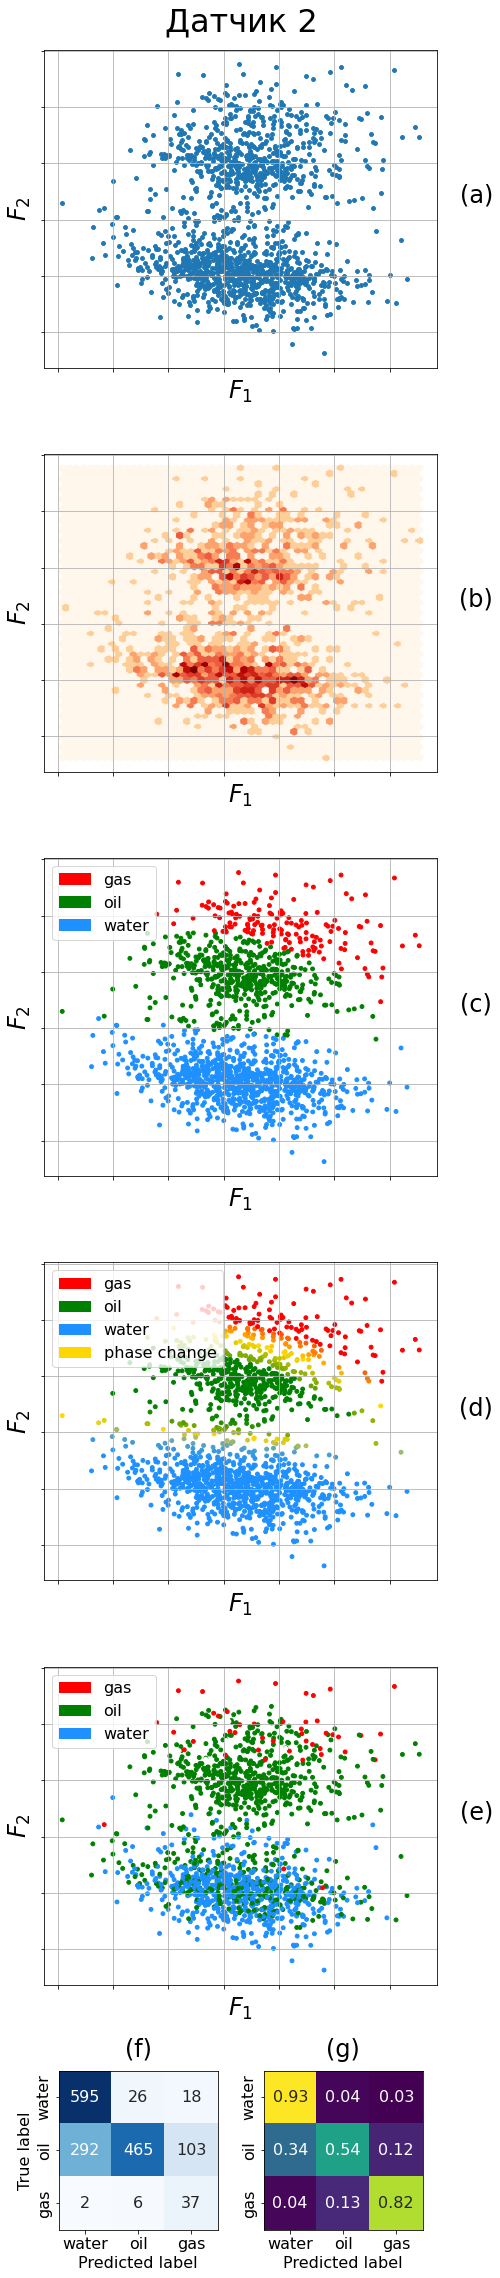
\includegraphics[width=0.3\textwidth]{TA/appendix_2.png}}
\subfloat[]{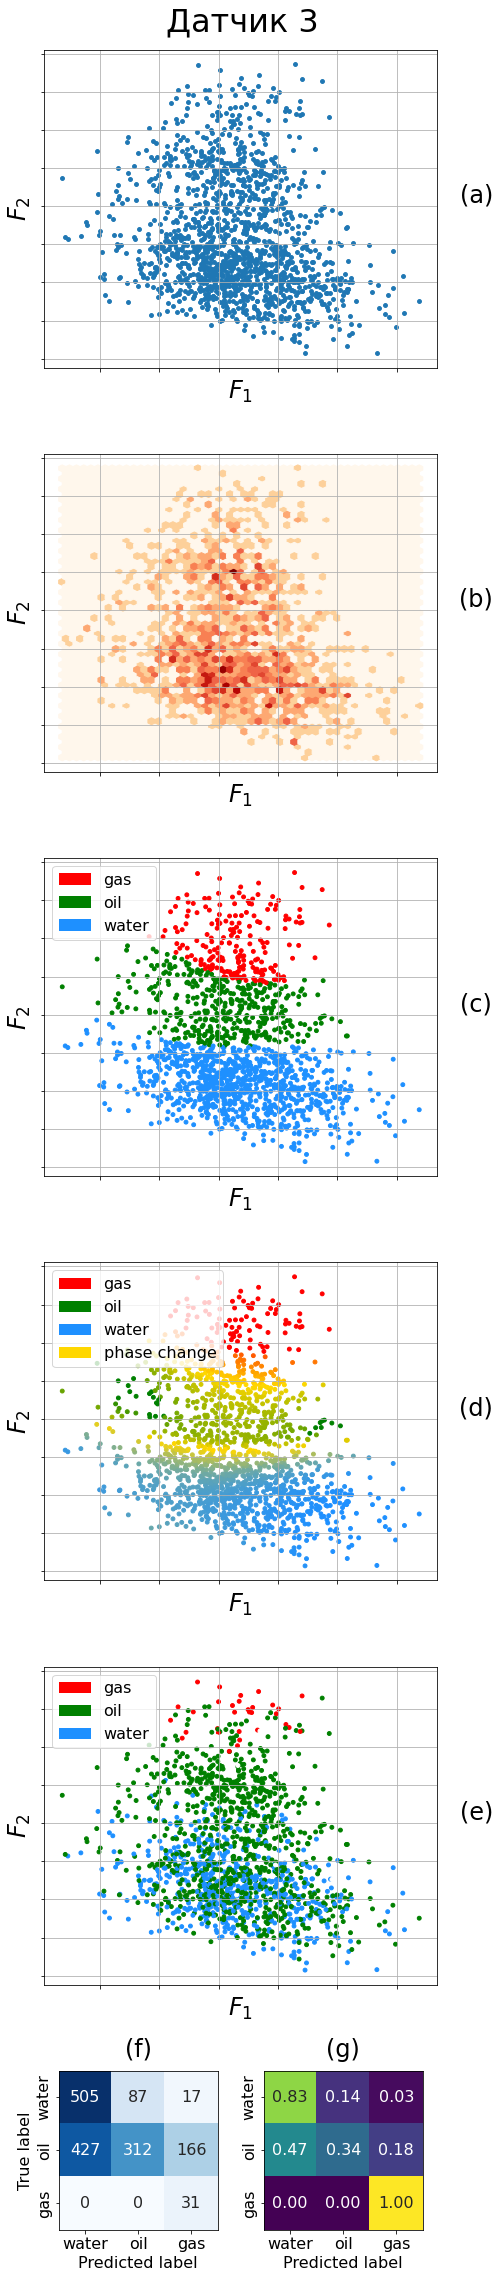
\includegraphics[width=0.3\textwidth]{TA/appendix_3.png}}
\caption{Датчики 1-3}
\label{fig:appendix_1}
\end{figure}

\newpage
\begin{figure}[H]
\centering
\subfloat[]{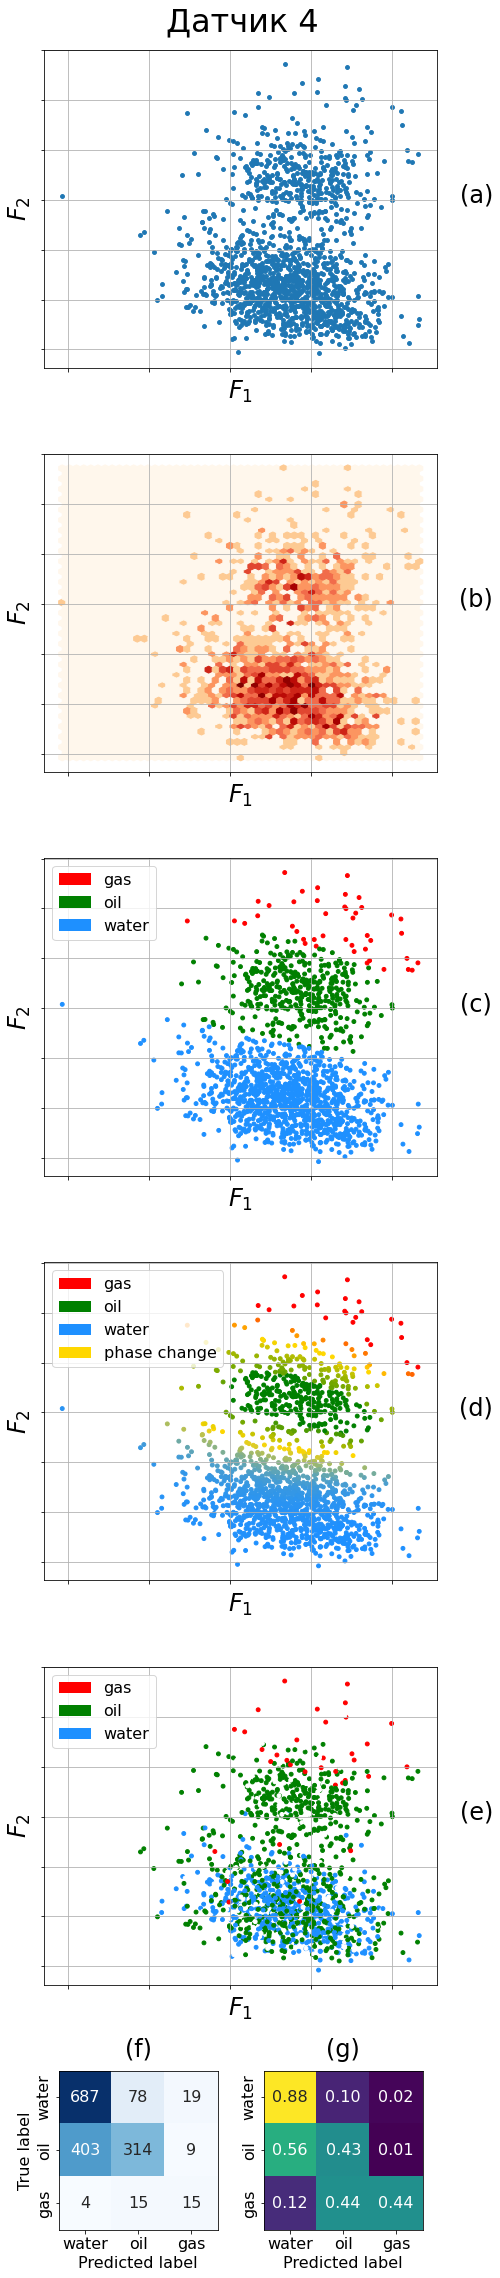
\includegraphics[width=0.3\textwidth]{TA/appendix_4.png}}
\subfloat[]{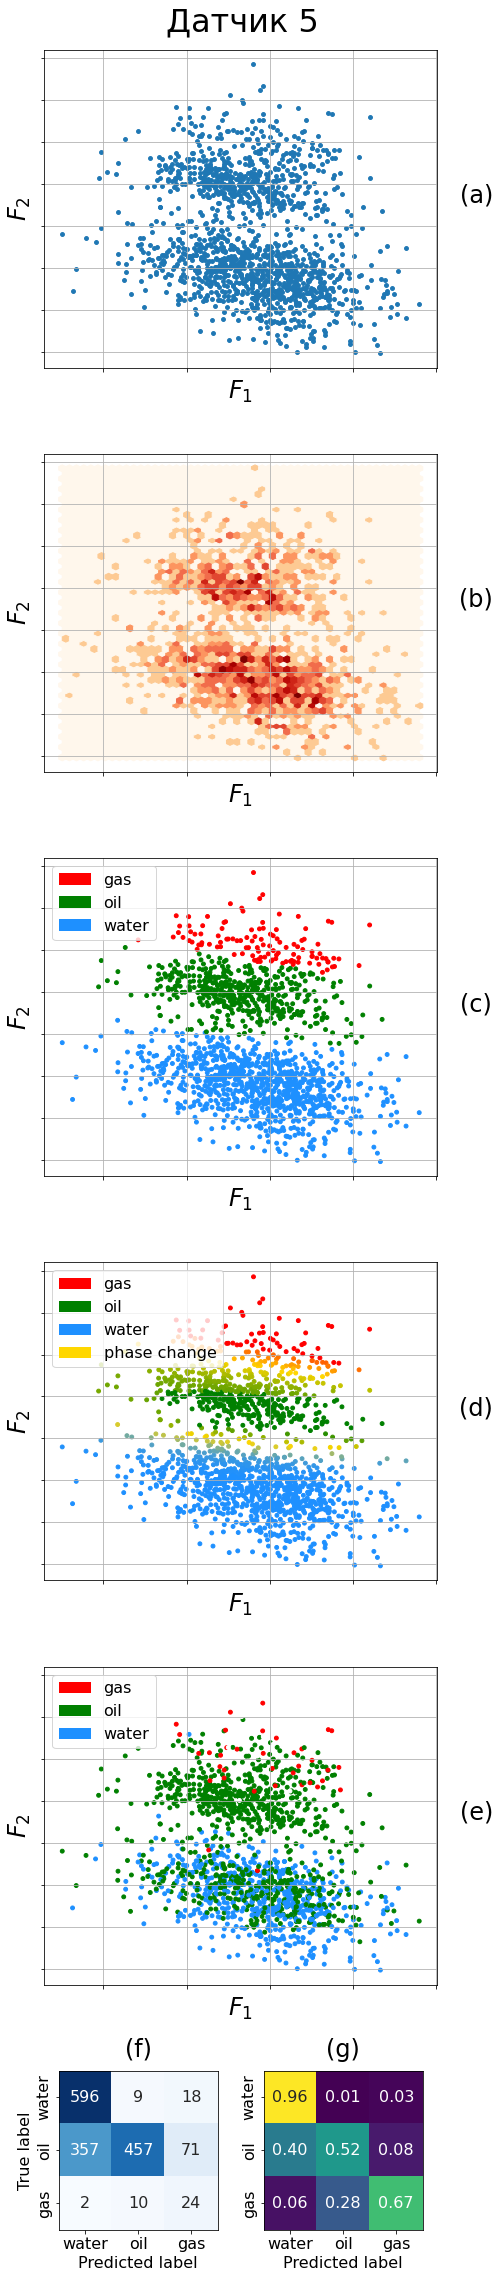
\includegraphics[width=0.3\textwidth]{TA/appendix_5.png}}
\subfloat[]{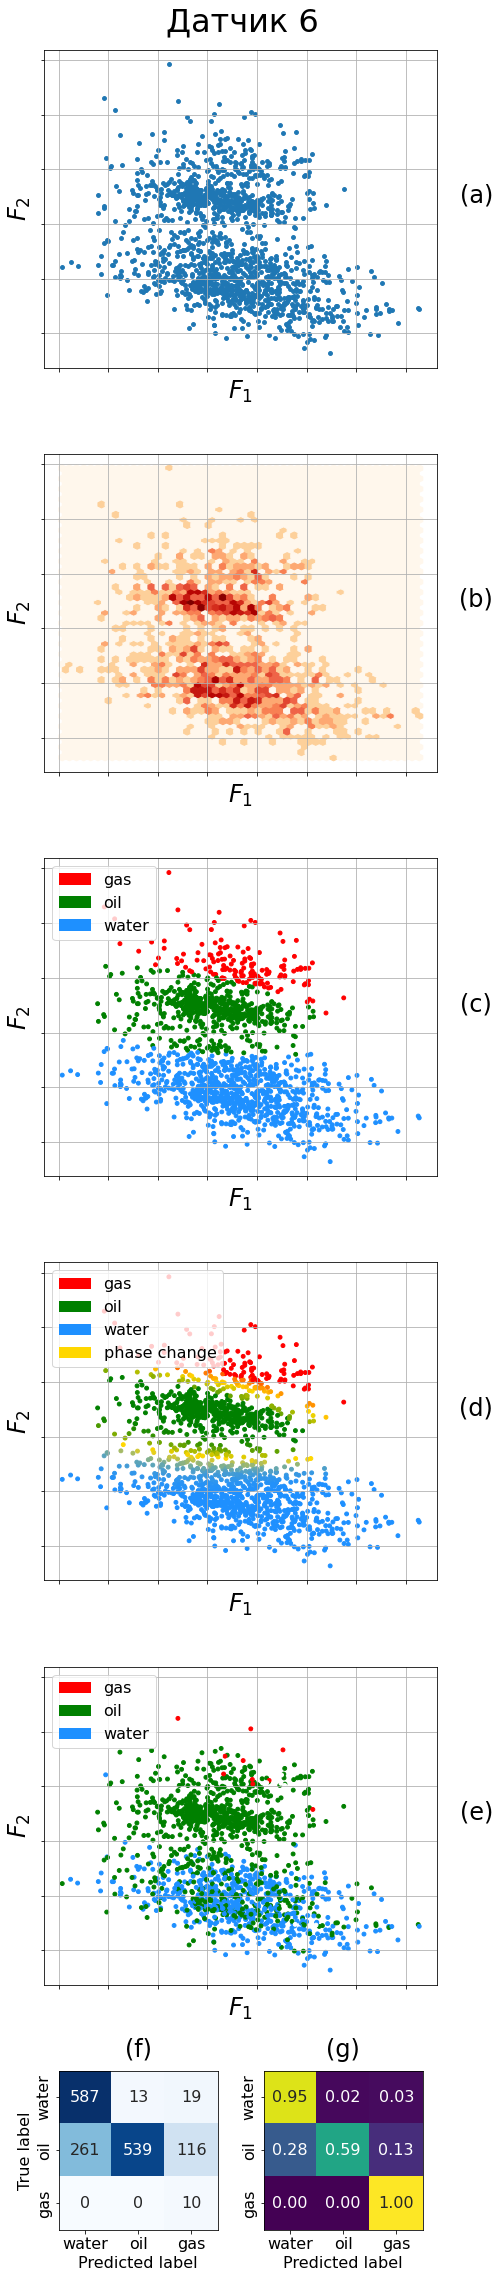
\includegraphics[width=0.3\textwidth]{TA/appendix_6.png}}
\caption{Датчики 4-5}
\label{fig:appendix_2}
\end{figure}